\documentclass[tikz,border=10pt]{standalone}
\usepackage{tikz}
\usepackage{fontawesome5}
\usepackage{amsmath,amssymb}
\usetikzlibrary{arrows.meta,positioning,fit,backgrounds,calc,shadows,shapes.geometric}

\definecolor{civNavy}{RGB}{15, 34, 64}
\definecolor{civBlue}{RGB}{28, 80, 160}
\definecolor{civTeal}{RGB}{14, 130, 120}
\definecolor{civLightBlue}{RGB}{238, 245, 255}
\definecolor{civGold}{RGB}{217, 119, 6}
\definecolor{civGreen}{RGB}{22, 130, 80}
\definecolor{civRed}{RGB}{220, 38, 38}
\definecolor{cInput}{RGB}{240, 246, 255}
\definecolor{cStem}{RGB}{224, 242, 254}
\definecolor{cStage1}{RGB}{209, 250, 229}
\definecolor{cStage2}{RGB}{254, 243, 199}
\definecolor{cStage3}{RGB}{254, 226, 226}
\definecolor{cStage4}{RGB}{236, 254, 255}

\begin{document}
% Complaint Lifecycle State Machine & Escalation DAG for CiviQ
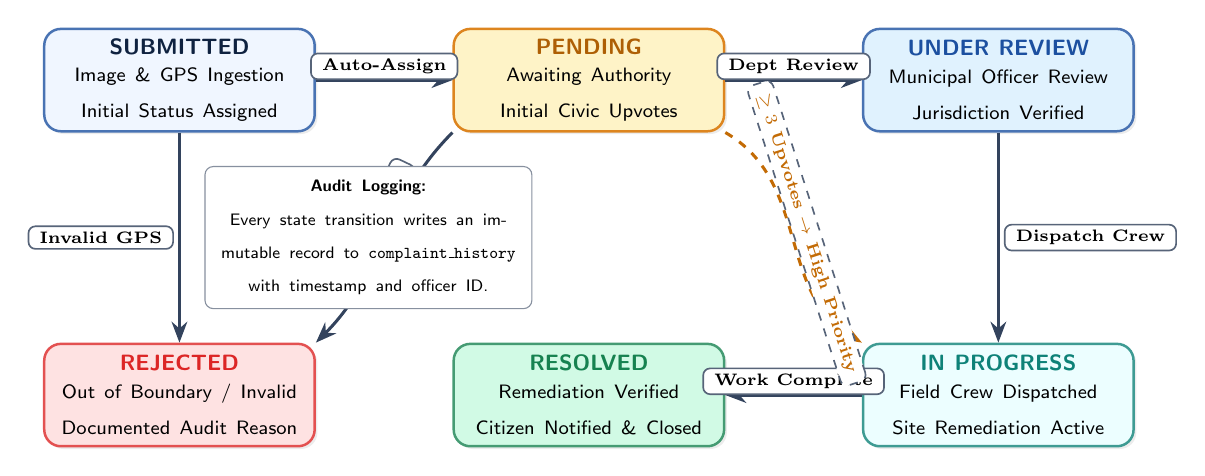
\begin{tikzpicture}[
    x=1cm, y=1cm,
    font=\sffamily,
    every node/.style={align=center},
    statebox/.style={
        rectangle, rounded corners=6pt, minimum width=3.4cm, minimum height=1.3cm,
        text width=3.2cm, align=center, line width=0.9pt, draw=civNavy!80, fill=white,
        drop shadow={shadow xshift=1pt, shadow yshift=-1pt, opacity=0.15}
    },
    transarr/.style={
        -{Stealth[scale=0.95]}, line width=1.1pt, draw=civNavy!85
    },
    esclarr/.style={
        -{Stealth[scale=0.95]}, line width=1.1pt, dashed, draw=civGold!90!black
    },
    auditbadge/.style={
        rectangle, rounded corners=2.5pt, fill=white, draw=civNavy!70, line width=0.6pt,
        inner xsep=4pt, inner ysep=2pt, font=\fontsize{6.0}{7.0}\selectfont\bfseries,
        align=center
    }
]

    % State Nodes
    \node (ssub) [statebox, fill=cInput, draw=civBlue!80] at (0, 6.0) {%
        \textbf{\fontsize{8.5}{10.0}\selectfont\color{civNavy}SUBMITTED}\\[0.2em]
        {\fontsize{6.8}{8.0}\selectfont Image \& GPS Ingestion\\[1pt]Initial Status Assigned}%
    };

    \node (spen) [statebox, fill=cStage2, draw=civGold!90] at (5.2, 6.0) {%
        \textbf{\fontsize{8.5}{10.0}\selectfont\color{civGold!80!black}PENDING}\\[0.2em]
        {\fontsize{6.8}{8.0}\selectfont Awaiting Authority\\[1pt]Initial Civic Upvotes}%
    };

    \node (srev) [statebox, fill=cStem, draw=civBlue!80] at (10.4, 6.0) {%
        \textbf{\fontsize{8.5}{10.0}\selectfont\color{civBlue}UNDER REVIEW}\\[0.2em]
        {\fontsize{6.8}{8.0}\selectfont Municipal Officer Review\\[1pt]Jurisdiction Verified}%
    };

    \node (sprog) [statebox, fill=cStage4, draw=civTeal!80] at (10.4, 2.0) {%
        \textbf{\fontsize{8.5}{10.0}\selectfont\color{civTeal}IN PROGRESS}\\[0.2em]
        {\fontsize{6.8}{8.0}\selectfont Field Crew Dispatched\\[1pt]Site Remediation Active}%
    };

    \node (sres) [statebox, fill=cStage1, draw=civGreen!80] at (5.2, 2.0) {%
        \textbf{\fontsize{8.5}{10.0}\selectfont\color{civGreen}RESOLVED}\\[0.2em]
        {\fontsize{6.8}{8.0}\selectfont Remediation Verified\\[1pt]Citizen Notified \& Closed}%
    };

    \node (srej) [statebox, fill=cStage3, draw=civRed!80] at (0, 2.0) {%
        \textbf{\fontsize{8.5}{10.0}\selectfont\color{civRed}REJECTED}\\[0.2em]
        {\fontsize{6.8}{8.0}\selectfont Out of Boundary / Invalid\\[1pt]Documented Audit Reason}%
    };

    % Transitions
    \draw [transarr] (ssub) -- node[above, auditbadge] {Auto-Assign} (spen);
    \draw [transarr] (spen) -- node[above, auditbadge] {Dept Review} (srev);
    \draw [transarr] (srev) -- node[right=2pt, auditbadge] {Dispatch Crew} (sprog);
    \draw [transarr] (sprog) -- node[above, auditbadge] {Work Complete} (sres);
    \draw [transarr] (ssub) -- node[left=2pt, auditbadge] {Invalid GPS} (srej);
    \draw [transarr] (spen.south west) to[out=225, in=45] node[pos=0.5, above, auditbadge, sloped] {Reject Claim} (srej.north east);

    % Escalation Path (from Pending to In Progress)
    \draw [esclarr] (spen.south east) to[out=-30, in=150] 
        node[pos=0.5, above, auditbadge, sloped, text=civGold!90!black] 
        {$\ge 3$ Upvotes $\rightarrow$ High Priority} (sprog.north west);

    % Legend Box in left-center zone (completely away from escalation arrow)
    \node (legend) [rectangle, draw=civNavy!50, rounded corners=3pt, fill=white, inner sep=5pt, align=center, text width=3.8cm] at (2.4, 4.0) {%
      {\fontsize{6.5}{7.8}\selectfont\textbf{Audit Logging:}\\Every state transition writes an immutable record to \texttt{complaint\_history} with timestamp and officer ID.}%
    };

\end{tikzpicture}
\end{document}
